\documentclass[main.tex]{subfiles}
\usepackage{amssymb}
\begin{document}

Los brazos robóticos ya son muy conocidos y utilizados pero el
valor agregado es la reconfiguracion/reprogramacion mediante un
brazo robótico a escala.

Indagar a nivel nacional la necesidad de las empresas, y presentarle
esta solución económica y reutilizable al ser de bajo costo y de alta
factibilidad.

Básicamente lo que se plantea es un brazo multifuncional, de esta manera
no hay necesidad de desechar un brazo, de esta manera disminuyendo el
impacto ambiental.


\subsection{Geometría 3D}
Para el desarrollo e implementación del código es necesario conocer
el modo de operación de las ecuaciones y funciones definidas. Por
tanto a continuación se muestran las definiciones y ecuaciones
previas al desarrollo del código.

\begin{itemize}
\item Puntos o vectores
  \begin{itemize}
  \item Vector
    \begin{equation}
      \mathbf{X} = \left(
      \begin{array}{ccc}x \\y \\z \\\end{array} \right)
      \epsilon \mathbb{R}^{3}
    \end{equation}
  \item Vector aumentado
    \begin{equation}
      \mathbf{\bar{X}} = \left(
          \begin{array}{ccc}x \\y \\z \\1 \\
          \end{array}        \right) \epsilon \mathbb{R}^{4}
    \end{equation}
  \item Coordenadas Homogéneas
    \begin{equation}
      \mathbf{\tilde{X}} = \left(
          \begin{array}{ccc}
            \tilde{x} \\ \tilde{y} \\ \tilde{z} \\ \tilde{w} \\
          \end{array}
        \right) \epsilon \mathbb{P}^{3}
    \end{equation}
  \end{itemize}
\item Rectas
  \begin{itemize}
  \item Recta sobre los puntos p y q
    \begin{equation}
      r = (1-\lambda )p+\lambda q
    \end{equation}
    \begin{equation}
      \lambda \epsilon \mathbb{R}
    \end{equation}
  \item Segmento de línea sobre p y q
    \begin{equation}
      r = (1-\lambda )p+\lambda q
    \end{equation}
    \begin{equation}
      0\leq \lambda  \leq 1
    \end{equation}
    \begin{figure}[h]
      \centering
      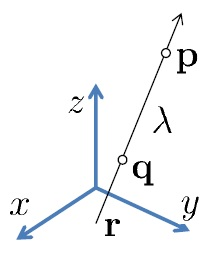
\includegraphics[width=0.2\textwidth]{../img/recta_3d.jpg}
      \caption{Recta 3D}
      \label{recta3d}
    \end{figure}
  \end{itemize}
\item Planos:
  \begin{itemize}
  \item Representación vectorial del plano
    \begin{equation}
      \tilde{m}=\left ( a,b,c,d \right )^{T}
    \end{equation}
  \item Ecuación del plano
    \begin{equation}
      \tilde{m}=\left ( a,b,c,d \right )^{T}    
    \end{equation}
  \item Plano normalizado con vector unitario normal “n” y distancia “d”
    \begin{equation}
      m= \left( \hat{n_{x}},\hat{n_{y}},\hat{n_{z}},d \right) ^ {T}=
         \left( \hat{n},d \right)
    \end{equation}
    \begin{equation}
      \left \| \hat{n} \right \| = 1
    \end{equation}
    \begin{figure}[h]
      \centering
      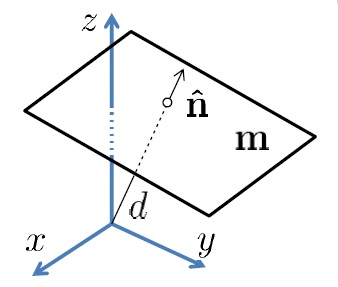
\includegraphics[width=0.2\textwidth]{../img/plano_3d.jpg}
      \caption{Recta 3D}
      \label{recta3d}
    \end{figure}
  \end{itemize}
\end{itemize}

\end{document}
